\begin{figure}[h!]
\centering
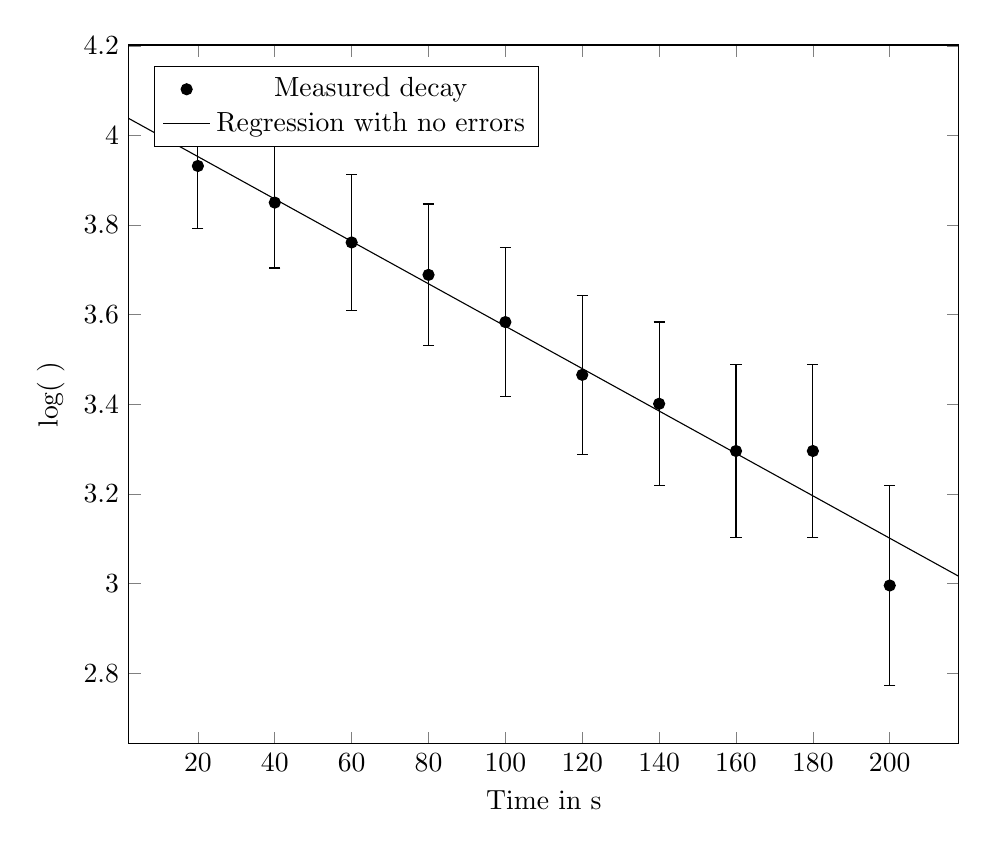
\begin{tikzpicture}
\begin{axis}
[ xlabel = Time in s,
ylabel = log( \symN ),
legend pos = north west,
xmin=2, xmax=218,
ymin=2.6421528, ymax=4.2018266,
width=1\textwidth
]
\addplot[
only marks,
error bars/.cd,
 y dir=both,y explicit,
x dir=both,x explicit,
]
coordinates{
(20,3.9318256327243257) +- (0,0.140028008402801)
(40,3.8501476017100584) +- (0,0.14586499149789456)
(60,3.7612001156935624) +- (0,0.15249857033260467)
(80,3.6888794541139363) +- (0,0.15811388300841897)
(100,3.58351893845611) +- (0,0.16666666666666666)
(120,3.4657359027997265) +- (0,0.1767766952966369)
(140,3.4011973816621555) +- (0,0.18257418583505539)
(160,3.295836866004329) +- (0,0.19245008972987526)
(180,3.295836866004329) +- (0,0.19245008972987526)
(200,2.995732273553991) +- (0,0.223606797749979)
};
\addlegendentry{Measured decay}
\addplot[
domain=2:218,
]
{x*-0.004731109358766987 + 4.04741313273662}
;
\addlegendentry{Regression with no errors}
\end{axis}
\end{tikzpicture}
\caption{Decay of Ba-137}
\label{fig:BaDecay}
\end{figure}
